\documentclass[openany, 12pt]{book}
\makeindex

\usepackage{amsmath}
\usepackage{amssymb}
\usepackage{booktabs}
\usepackage[dvipsnames]{xcolor}
\usepackage{enumitem}
\usepackage[toc]{glossaries}
\usepackage{graphicx}
\usepackage[citecolor=blue,colorlinks=true, linkcolor=blue, urlcolor=blue]{hyperref}
\usepackage{makeidx}
\usepackage[margin=0.8in]{geometry}
\usepackage{mathrsfs}
\usepackage{minted}
\usepackage{multicol}
\usepackage[style=authortitle]{biblatex}
\usepackage[T1]{fontenc}
\usepackage{tcolorbox}
\usepackage{tikz}
\usepackage{titlesec}
\usepackage{xcolor}

\usetikzlibrary{arrows}
\usetikzlibrary{arrows.meta}
\usetikzlibrary{automata}
\usetikzlibrary{calc}
\usetikzlibrary{fit}
\usetikzlibrary{petri}
\usetikzlibrary{positioning}

\tcbuselibrary{breakable}
\tcbuselibrary{listings}
\tcbuselibrary{minted}
\tcbuselibrary{skins}
\tcbuselibrary{theorems}

\newcounter{filePrg}

% \addbibresource{biblio.bib}
\setlength{\parindent}{0pt}

\renewcommand{\emph}[1]{\textit{#1}}
\setlength{\parindent}{0pt}

\newcommand\setboxcounter[2]{\setcounter{tcb@cnt@#1}{#2}}
\setlength{\parindent}{10pt}
\newcommand{\set}[1]{\{#1\}}

\definecolor{CaribbeanBlue}{RGB}{0, 206, 209} % Define Caribbean Blue
\NewTcbTheorem[list inside=definition]{definition}
{Definition}{
	breakable,
	colback=CaribbeanBlue!05,
	colframe=CaribbeanBlue!35!black,
	fonttitle=\bfseries}{th}

\NewTcbTheorem[list inside=intuition]{intuition}{Intuition}{
	breakable,
	colback=blue!5,
	colframe=blue!35!black,
	fonttitle=\bfseries}{th}

\NewTcbTheorem{example}{Example}{
	breakable,
	colback=white,
	colframe=green!35!black,
	fonttitle=\bfseries}{th}

\NewTcbTheorem{verify}{Verify}{
	breakable,
	float,
	colback=red!5,
	colframe=red!35!black,
	fonttitle=\bfseries}{th}

\NewTcbTheorem[list inside=theorem]{theorem}{Theorem}{
	breakable,
	colback=gray!10,
	colframe=gray!35!black,
	fonttitle=\bfseries}{th}

\NewTcbTheorem[
	list inside=exercise,
	number within=section
]
{exercise}{Exercise}{
	breakable,
	colback=white,
	colframe=black,
	fonttitle=\bfseries}{th}

\newcommand{\hask}[1]{\mintinline{haskell}{#1}}

\newenvironment{alist}
{\begin{enumerate}[label={*}, leftmargin=*, itemsep=0pt, parsep=0pt]}
		{\end{enumerate}}

\newenvironment{blist}
{\begin{enumerate}[label={}, leftmargin=*, itemsep=0pt, parsep=0pt]}
		{\end{enumerate}}


\renewcommand{\thesection}{\arabic{section}}
\tcbset{enhanced jigsaw}

\newtcbinputlisting{\codeFromFile}[2]{
	listing file={#1},
	listing engine=minted,
	minted style=colorful,
	minted language=haskell,
	minted options={breaklines,linenos,numbersep=3mm},
	colback=blue!5!white,colframe=blue!75!black,listing only,
	left=5mm,enhanced,
	title={#2},
	overlay={\begin{tcbclipinterior}\fill[red!20!blue!20!white] (frame.south west)
				rectangle ([xshift=5mm]frame.north west);\end{tcbclipinterior}}
}

\newtcblisting{haskell}[1]
{
	listing engine=minted,
	minted style=colorful,
	minted language=haskell,
	minted options={breaklines,linenos,numbersep=3mm},
	colback=blue!5!white,colframe=blue!75!black,listing only,
	left=5mm,enhanced,
	title={#1},
	overlay={\begin{tcbclipinterior}\fill[red!20!blue!20!white] (frame.south west)
				rectangle ([xshift=5mm]frame.north west);\end{tcbclipinterior}}
}

\newtcblisting{shell}[1]
{
	listing engine=minted,
	minted style=colorful,
	minted language=shell,
	minted options={breaklines,linenos,numbersep=3mm},
	colback=blue!5!white,colframe=blue!75!black,listing only,
	left=5mm,enhanced,
	title={#1},
	overlay={\begin{tcbclipinterior}\fill[red!20!blue!20!white] (frame.south west)
				rectangle ([xshift=5mm]frame.north west);\end{tcbclipinterior}}
}

\title{Haskell Tooling}
\author{Idris}
\date{August 2025}

%chktex-file 1

\newglossaryentry{mesa} {
	name=mesa,
	description={Collection of userspace GPU drivers that implement APIs like OpenGL, Vulkan, and OpenCL, translating them into GPU commands on Linux}
}


\newglossaryentry{KMS} {
	name=kms,
	description={Kernel Mode Setting is the Linux kernel subsystem responsible
			for setting display resolution, refresh rate, and managing video
			outputs. It enumerates your displays and sets properties such as their
			selected resolution, also known as their ``mode''
		}
}

\newglossaryentry{DRM} {
	name=drm,
	description={Direct Rendering Manager is the Linux kernel subsystem that
			manages GPU access, buffer objects, and rendering synchronization. It
			efficiently tasks the GPU with work from userspace
		}
}

\newglossaryentry{EGL} {
	name=EGL,
	description={
			Interface between rendering APIs (like OpenGL or OpenGL ES) and the
			native platform windowing system, used to create GPU contexts and
			manage rendering surfaces
		}
}


\newglossaryentry{GBM} {
	name=gbm,
	description={Generic Buffer Management is a userspace library that lets
			applications allocate GPU buffers for rendering without a window system}
}

\newglossaryentry{libdrm} {
	name=libdrm,
	description={userspace library that wraps DRM ioctls, providing
			Mesa and other clients safe access to the kernel’s graphics APIs}
}

\newglossaryentry{libinput} {
	name=libinput,
	description={library that handles input device events like
			touchpads, keyboards, and mice in a compositor-friendly, unified way}
}

\newglossaryentry{evdev} {
	name=evdev,
	description={(event device) is a Linux kernel interface that exposes
			input devices as event streams under \texttt{/dev/input/}}
}

\makeglossaries

% \usepackage{tikz-uml}
\begin{document}

\tableofcontents

\chapter{Introduction}


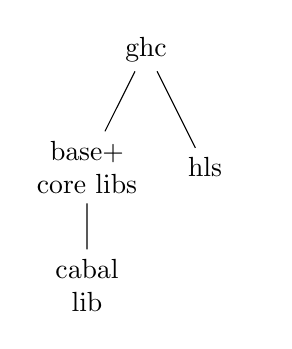
\begin{tikzpicture} [every node/.append style={
				grow=left,
				minimum width=15mm,
				align=center
			}]
	\node {ghc}
	child {node {base+\\core libs}
			child {node {cabal\\lib}}
		}
	child {node {hls}
		};
\end{tikzpicture}

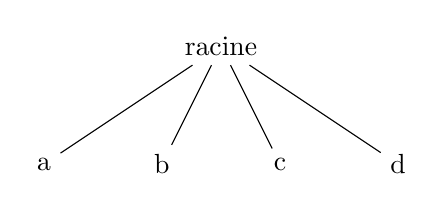
\begin{tikzpicture}
	\node {racine} child foreach \name in {a,b,c,d} {node {\name}};
\end{tikzpicture}


\begin{align*}
	A & :=\text{ghc}       \\
	B & :=\text{base}      \\
	C & :=\text{cabal lib} \\
	A & \implies B         \\
	A & \implies C         \\
\end{align*}

\chapter{stack}

\chapter{cabal}
Cabal is at least three things---a library, a cli app which uses the library,
and a specificiation for how to distribute haskell packages.

\begin{table}[h]
	\centering
	% \rowcolors{2}{blue!5}{white}
	\begin{tabular}{lll}
		\toprule
		{Cabal library} & {Bundled with GHC} & {GHC range supported} \\
		\midrule
		1.10            & 7.0                & 7.0 --- 7.4           \\
		1.14            & 7.6                & 7.6 --- 7.8           \\
		1.18            & 7.8                & 7.8 --- 7.10          \\
		1.22            & 7.10               & 7.10 --- 8.0          \\
		1.24            & 8.0                & 8.0 --- 8.2           \\
		2.0             & 8.2                & 8.2 --- 8.4           \\
		2.2             & 8.4                & 8.4 --- 8.6           \\
		2.4             & 8.6                & 8.6 --- 8.8           \\
		2.4.1           & 8.8                & 8.8 --- 8.10          \\
		3.0             & 8.10               & 8.10 --- 9.0          \\
		3.2             & 9.0                & 9.0 --- 9.2           \\
		3.4             & 9.2                & 9.2 --- 9.4           \\
		3.6             & 9.4                & 9.4 --- 9.6           \\
		3.8             & 9.6                & 9.6 --- 9.8           \\
		3.10            & 9.8                & 9.8 --- 9.10          \\
		3.12            & 9.10               & 9.10+                 \\
		\bottomrule
	\end{tabular}
	\caption{}
\end{table}

\chapter{haskell language server}

\begin{table}[h]
	\centering
	% \rowcolors{2}{blue!5}{white}
	\begin{tabular}{ll}
		\toprule
		\textbf{HLS Version} & \textbf{Supported GHC Versions}     \\
		\midrule
		2.11.0.0             & 9.4.8, 9.6.7, 9.8.4, 9.10.2, 9.12.2 \\
		2.10.0.0             & 9.4.8, 9.6.7, 9.8.4, 9.10.1         \\
		2.9.0.1              & 9.2.8, 9.4.8, 9.6.6, 9.8.2, 9.10.1  \\
		2.9.0.0              & 9.2.x, 9.4.x, 9.6.x, 9.8.1          \\
		2.8.0.0              & 9.2.x, 9.4.x, 9.6.2                 \\
		2.7.0.0              & 9.0.x, 9.2.x, 9.4.x                 \\
		2.6.0.0              & 8.10.x, 9.0.x, 9.2.x                \\
		\bottomrule
	\end{tabular}
	\caption{Haskell Language Server versions and their GHC compatibility}
\end{table}


\chapter{ghc}

\begin{table}[h]
	\centering
	% \rowcolors{2}{blue!5}{white} % alternate row coloring
	\begin{tabular}{llll}
		\toprule
		Major & Minor & base version & Release date \\
		\midrule
		7     & 0     & 4.3          & 2010 Nov     \\
		7     & 2     & 4.4          & 2011 Aug     \\
		7     & 4     & 4.5          & 2012 Jan     \\
		7     & 6     & 4.6          & 2012 Sep     \\
		7     & 8     & 4.7          & 2014 Apr     \\
		7     & 10    & 4.8          & 2015 Mar     \\
		8     & 0     & 4.9          & 2016 May     \\
		8     & 2     & 4.10         & 2017 Jul     \\
		8     & 4     & 4.11         & 2018 Mar     \\
		8     & 6     & 4.12         & 2018 Sep     \\
		8     & 8     & 4.13         & 2019 Aug     \\
		8     & 10    & 4.14         & 2020 Apr     \\
		9     & 0     & 4.15         & 2021 Feb     \\
		9     & 2     & 4.16         & 2021 Nov     \\
		9     & 4     & 4.17         & 2022 Aug     \\
		9     & 6     & 4.18         & 2023 Mar     \\
		9     & 8     & 4.19         & 2023 Nov     \\
		9     & 10    & 4.20         & 2024 Aug     \\
		9     & 12    & 4.21         & 2025 Jan     \\
		\bottomrule
	\end{tabular}
	\caption{GHC version with base and release date}
\end{table}

\chapter{nixpkgs}
\chapter{haskell.nix}
\chapter{stackage.nix}
\chapter{external libs}

\clearpage
\printglossaries

% \printbibliography{}
\printindex{}
\end{document}
